\documentclass[a4paper,11pt]{article}

\usepackage[english]{babel} 
\usepackage[utf8]{inputenc}
\usepackage[cyr]{aeguill}
\usepackage{stmaryrd}

\usepackage{lmodern} %Type1-font for non-english texts and characters
\usepackage{caption}
\usepackage{subcaption}

\usepackage{graphicx}
\usepackage{hyperref}

\usepackage{epstopdf}


%\hypersetup{	
%colorlinks=true,   %colorise les liens 
%breaklinks=true,  %permet le retour à la ligne dans les liens trop longs 
%urlcolor= blue,    %couleur des hyperliens 
%linkcolor= black, %couleur des liens internes 
%citecolor=black,	 %couleur des références 
%pdftitle={Compte rendu \emph{Traitement numérique du signal}, %informations apparaissant dans 
%pdfauthor={Mélisande Zonta}, %les informations du document 
%pdfsubject={Projet TNS2}	%sous Acrobat. 
%} 

%% Math Packages 
\usepackage{amsmath}
\usepackage{amsthm}
\usepackage{amsfonts}
\usepackage{amssymb}
\usepackage{mathrsfs}
\usepackage{pst-all}
\usepackage{lscape}
\usepackage{pdfpages}
\usepackage{mathabx}


\usepackage{color, colortbl}
\definecolor{lightgray}{gray}{0.85}
\usepackage{multirow}
\usepackage[Algorithme]{algorithm}
\usepackage[noend]{algpseudocode}
\usepackage{tikz}

%\renewcommand{\algorithmicdo}{\textbf{faire}}
%\renewcommand{\algorithmicwhile}{\textbf{tant que}}


\usepackage{a4wide} %%Smaller margins = more text per page.
\usepackage{fancyhdr} %%Fancy headings

\setcounter{secnumdepth}{5}
\setcounter{tocdepth}{5}


\DeclareMathOperator*{\argmax}{arg\,max}
\DeclareMathOperator*{\argmin}{arg\,min}
\graphicspath{{/Users/melisandezonta/Documents/Documents/GTL_courses_second_semester/Computer-Vision/PS1-all/PS1-images/}}

\begin{document}

%\pagestyle{fancy}

\begin{titlepage}
\vspace*{\stretch{1}}

\begin{center}

\includegraphics[scale=0.4]{GT_logo.jpeg}
\end{center}
\vspace*{\stretch{1}}
\hrulefill
\begin{center}\bfseries\huge
   Computer Vision \\
   CS 6476 , Spring 2018\\
   \end{center}
  \begin{center}\bfseries\large
     PS 1\\
    \hrulefill
\end{center}
%\hfill
\vspace*{1cm}
\begin{minipage}[t]{0.6\textwidth}
  \begin{flushleft} \large
    \emph{Supervisor : }\\
    Cedric Pradalier \\
  \end{flushleft}
\end{minipage}
\begin{minipage}[t]{0.3\textwidth}
  \begin{flushright} \large
    \emph{Author :} \\
    Melisande Zonta \\
  \end{flushright}
\end{minipage}
\vspace*{\stretch{2}}
\begin{flushright}
       \today 
\end{flushright} 
\end{titlepage}

\tableofcontents
\clearpage

\section{Creation of the edges image}



 \begin{figure}[H]
\begin{center}
\begin{tabular}{cc}
	
\includegraphics[height=.3\textwidth]{ps1-1-a-original.png}&
	
\includegraphics[height=.3\textwidth]{ps1-1-a-edges.png}\\
	a&b
\end{tabular}
\end{center}
\caption{ 
\textit{a}. ps1-1-a : Original Image. \textit{b}. ps1-1-a : Edges Image.}
\label{ps1-1-a}
\end{figure}

The Figure 1 shows the result of our initial edge detection using the Canny edge detector.

\section{Hough Method applied on the lines}

 \begin{figure}[H]
\begin{center}
\begin{tabular}{cc}
	
\includegraphics[height=.4\textwidth]{ps1-1-a-original.png}&
	
\includegraphics[height=.4\textwidth]{ps1-2-edges.png}\\
	a&b\\
	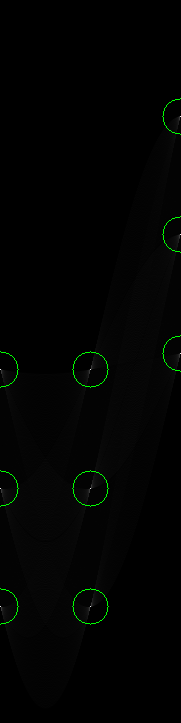
\includegraphics[height=.4\textwidth]{ps1-2-accu-circled.png}&
	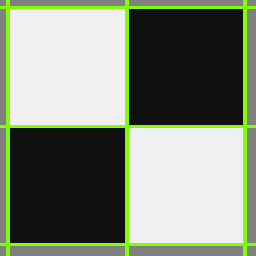
\includegraphics[height=.4\textwidth]{ps1-2-lines.png}\\
	c&d\\
\end{tabular}
\end{center}
\caption{ 
\textit{a}. ps1-2-original : Original Image.  \textit{b}. ps1-2-edges : Edges Image. \\
\textit{c}. ps1-2-accumulator : Hough accumulator array image. \textit{d}. ps1-2-lines : Intensity Image with lines drawn on them.}
\label{ps1-2}
\end{figure}

The Figure 2 shows the result of the voting in the accumulator and the associated image with the detected lines is shows in Figure 3.
Since the computation for this image is rather quick, we choose to keep a bin size of 1 degree on the theta parameter, to get a fine detection.
   
The image being a 256px square, the maximum value of d is the diagonal, around 136. Thus we choose a bin size of 180 on the d parameter, resulting in a rectangular accumulator.


\section{Noise effect on the lines detection}


\subsection{First Step : Smoothing}

\begin{figure}[H]
\centering
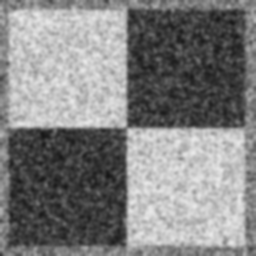
\includegraphics[height = .4\textwidth]{ps1-3-a-image-noisy-smoothed.png}
 \caption{ps1-3-a : Image noisy smoothed }
\label{ps1-3-a}
\end{figure}


The smoothed version using a Gaussian kernel is visible in Figure 3.


\subsection{Second Step : Edges detection}


 \begin{figure}[H]
\begin{center}
\begin{tabular}{cc}

\includegraphics[height  = .4\textwidth]{ps1-3-b-edges.png}&
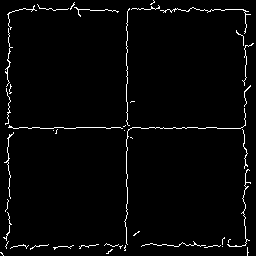
\includegraphics[height = .4\textwidth]{ps1-3-b-edges-image-noisy.png}\\
	a&b
\end{tabular}
\end{center}
 \caption{\textit{a}. ps1-3-b-original : Edges Original Image.  \textit{b}. ps1-3-b-noisy : Edges Smoothed Image. }
\label{ps1-3-b}
\end{figure}

The edges resulting from the Canny edge detector on the original image are shown in Figure 4.a, while those detected on the noisy image are visible in Figure 4.b.

\subsection{Third Step : Hough Algorithm for lines}

 \begin{figure}[H]
\begin{center}
\begin{tabular}{cc}
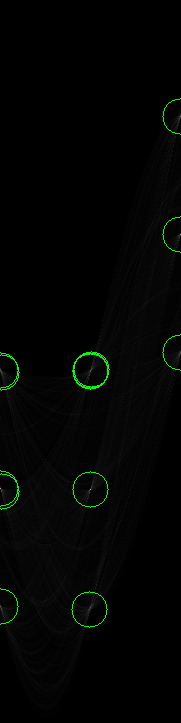
\includegraphics[height = .5\textwidth]{ps1-3-c-accu-circled.png}&
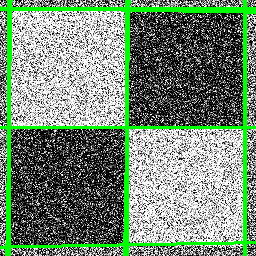
\includegraphics[height = .5\textwidth]{ps1-3-c-lines.png}\\
	a&b
\end{tabular}
\end{center}
 \caption{
\textit{a}. ps1-3-c-accumulator : Hough accumulator array image.  \textit{b}. ps1-3-c-lines : Intensity Image with lines drawn on them. }
\label{ps1-3-c}
\end{figure}

In order to get a good result, we first had to convolve the image with a standard 3x3 Gaussian kernel in order to get an image smoothed with a sigma of a few pixels.

Afterwards, we used the Canny edge detector in order to get a relatively good quality of edges, meaning at least getting each of the 6 edges about halfway visible on the edge image. Even if some artifacts are still visible, in will not matter much since the majority of edges still lie on a line.

I finally used the Hough line detection method to extract the 6 edges, which required lowering the threshold to get all of them. We see on Figure 5.b that vertical edges are represented by multiple lines instead of a single one. This is due to the fact that peaks on the edge of the theta axis get wrapped around the matrix and detected twice). This results in several lines with a little difference in angle.

\section{Lines detection on a more complicated image}

\subsection{First Step : Smoothing}

\begin{figure}[H]
\centering
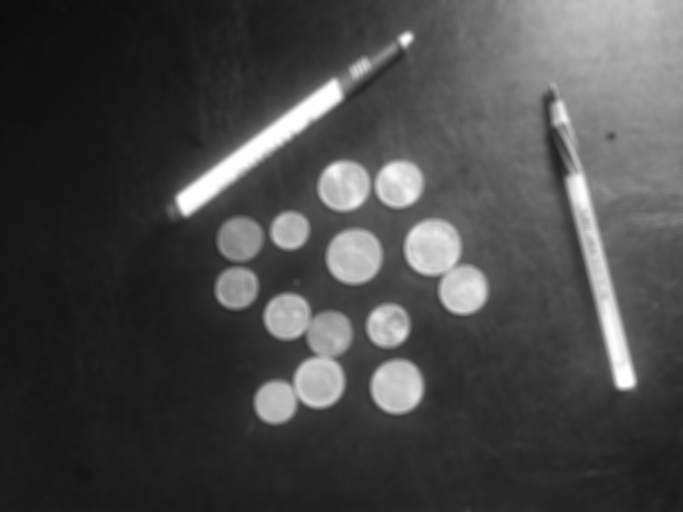
\includegraphics[width = .5\textwidth]{ps1-4-a-image-noisy-smoothed.png}
 \caption{ps1-4-a : Image noisy smoothed }
\label{ps1-4-a}
\end{figure}


The smoothed version of the pens and coins is visible in Figure 6.

\subsection{Second Step : Edges detection}


\begin{figure}[H]
\centering
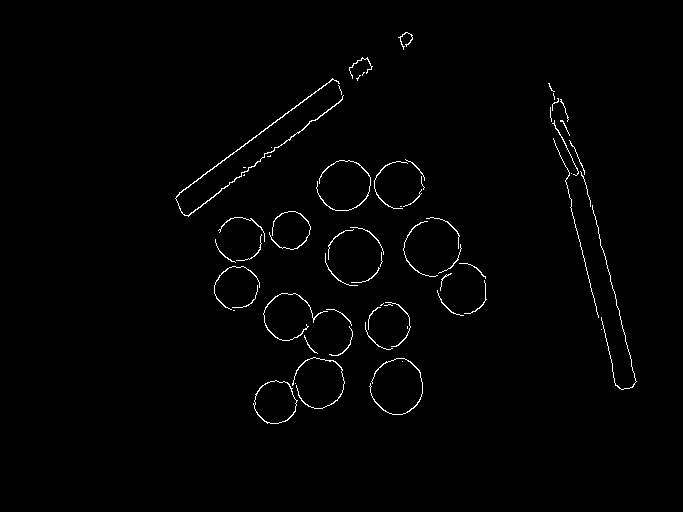
\includegraphics[width = .5\textwidth]{ps1-4-b-image-noisy-edges.png}
 \caption{ps1-4-b : Edges Smoothed Image }
\label{ps1-4-b}
\end{figure}

The Canny edge detection result is given in Figure 7.

\subsection{Third Step : Hough Algorithm for lines}

 \begin{figure}[H]
\begin{center}
\begin{tabular}{cc}

\includegraphics[height = .5\textwidth]{ps1-4-c-accu-circled.png}&
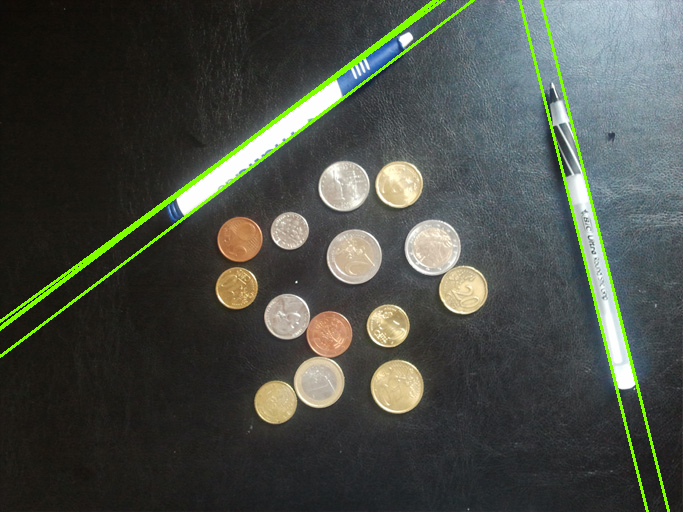
\includegraphics[height = .5\textwidth]{ps1-4-c-lines.png}\\
	a&b
\end{tabular}
\end{center}
 \caption{
\textit{a}. ps1-4-c-accumulator : Hough accumulator array image.  \textit{b}. ps1-4-c-lines : Intensity Image with lines drawn on them. }
\label{ps1-4-c}
\end{figure}

In order to get to the cleanly detected lines of the pens (Figure 8.b), we had to follow a similar process as previously.

This time we used a larger Gaussian kernel to get a wider extent of smoothing in order to avoid detecting any of the inner edges of the pens. The circles of the coins are less of a problem once we manage to keep them clean, since our Hough algorithm will target specifically the lines.

The resulting accumulator visible in Figure 8.a shows pair of peaks, corresponding to the parallel edges of the pens. We have twice the number of peaks as what is expected, since they are spaced of 180 degrees and result in superposing lines on the final image.

\section{Circles Detection}

 \begin{figure}[H]
\begin{center}
\begin{tabular}{cc}
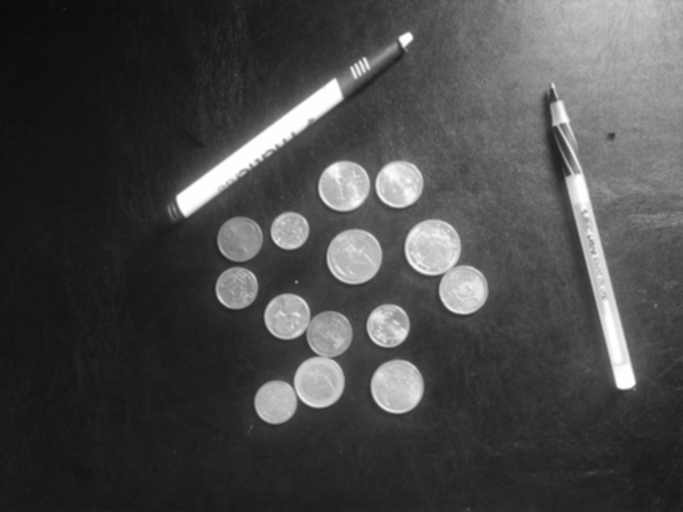
\includegraphics[width = .5\textwidth]{ps1-5-image-noisy-smoothed.png}&
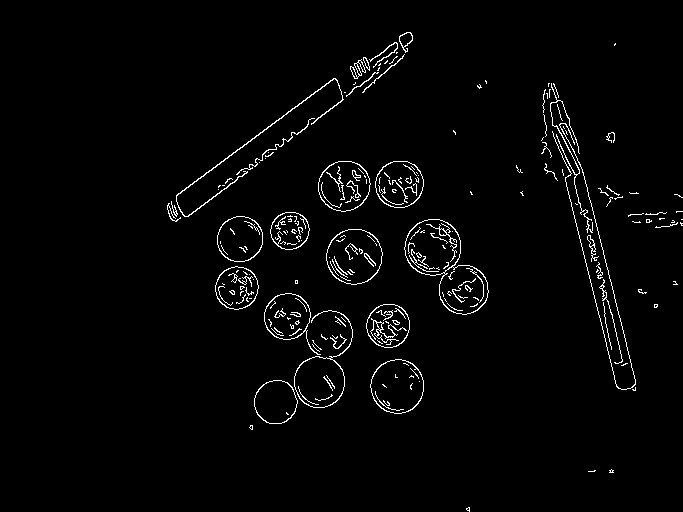
\includegraphics[width= .5\textwidth]{ps1-5-edges-image-noisy.png}\\
	a&b\\
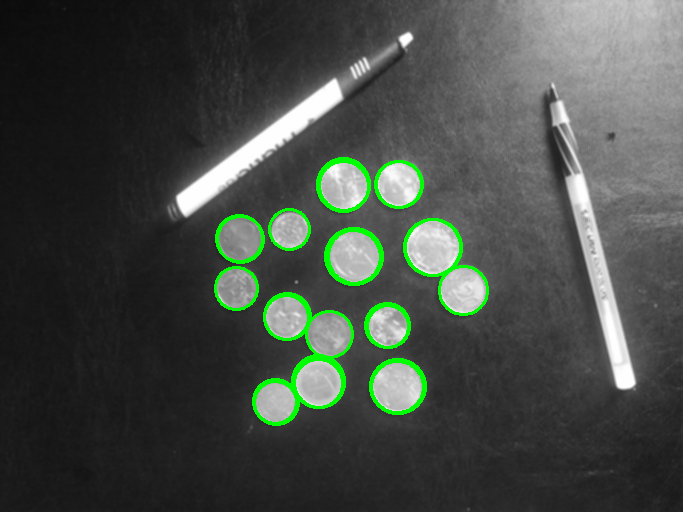
\includegraphics[width = .5\textwidth]{ps1-5-circles.png}\\
c
\end{tabular}
\end{center}
 \caption{
\textit{a}. ps1-5-smoothed : Image Noisy Smoothed.  \textit{b}. ps1-5-edges : Edges Smoothed Image.
\textit{c}. ps1-5-circles : Image with circles drawn in color. }
\label{ps1-5}
\end{figure}

In order to detect the coins, we need to adapt the Hough transform to circles. We change our Hough space parameters, from polar coordinates to 3 parameters: the cartesian coordinates of the circle center and the radius of the circle.

We use a slightly lighter smoothing than for the pen detection, since we do not care about their inner edges anymore (none of them is circular). We also use the same Canny edge detector parameters, which gives us the edges visible in Figure 9.b.

We estimate the radius of the coins to be between 15 and 30 pixels, which is necessary in order to limit the computation time of our algorithm. This is also something the standard OpenCV Hough detector offers.

For each edge point and each radius, we first computed the coordinates of the center for 180 values but in order to reduce the length of the computation an improvement of the algorithm was made by using the gradient to ?orient? the search for a potential center.
We finally filter the circles using an extra parameter which gives the minimum distance between two centers, thus avoiding concentric circles (which are not among our targets for this application) and also filtering the closeby maximas.
We get the resulting image shown in Figure 9.c.

\section{Finding lines on a more realistic image}

\subsection{Application on a line finder}


In the Figure 10.b are displayed the lines initially detected by our Hough transform (after a good smoothing to put aside the numerous edges of the text and barcode).

 \begin{figure}[H]
\begin{center}
\begin{tabular}{cc}
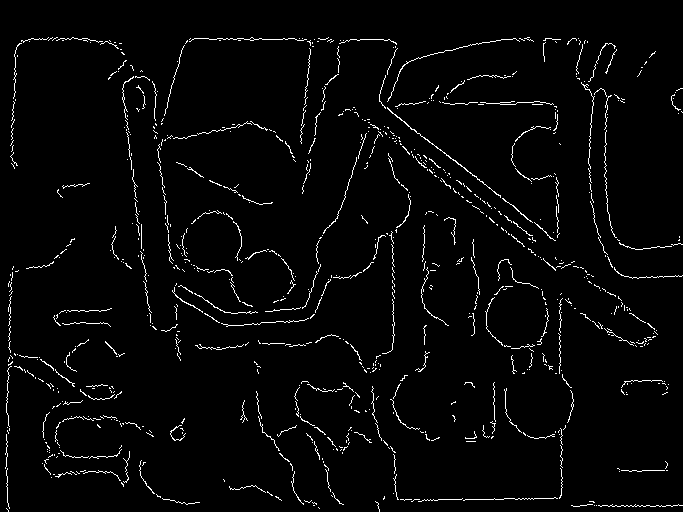
\includegraphics[width = .5\textwidth]{ps1-6-a-edges.png}&
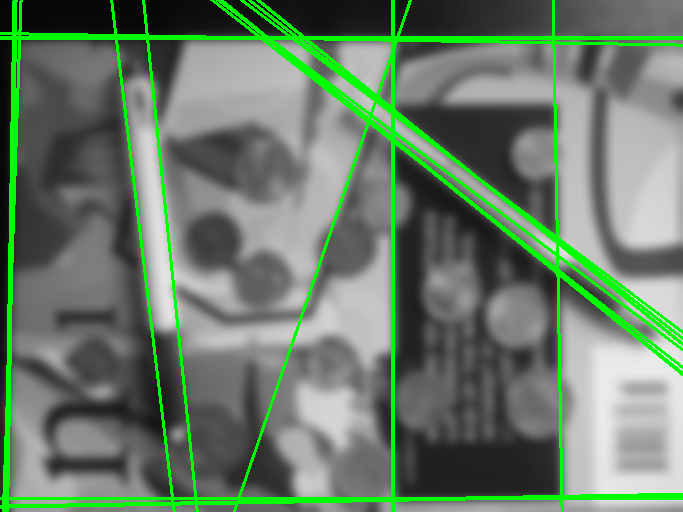
\includegraphics[width= .5\textwidth]{ps1-6-a-lines.png}\\
	a&b
\end{tabular}
\end{center}
 \caption{
\textit{a}. ps1-6-a-edges : Edges Image Smoothed.  \textit{b}. ps1-6-a-lines : Hough Lines drawn on the smoothed image.}
\label{ps1-6}
\end{figure}

\subsection{Problems with our line finder}

We note that many lines are rightfully detected by the algorithm because of the magazine cover borders and geometric content. However, we successfully avoided any of the smaller text and barcode edges.

As explained in the previous section, we will rely on the fact that the pens are composed of parallel edges, spaced by a certain amount of pixels, to filter out the undesirable edges.

\subsection{Attempt to find the boundaries lines of the pen}


Applying a maximum distance and specifying the maximum angle between two lines to be considered parallel, we manage to extract the pens boundaries as visible in Figure 11.

\begin{figure}[H]
\centering
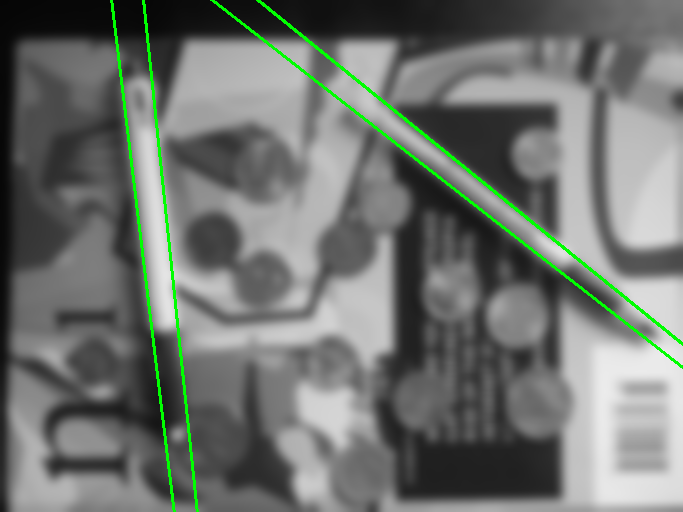
\includegraphics[width = .5\textwidth]{ps1-6-c-lines.png}
 \caption{ps1-6-c :New Hough lines drawn on the smoothed image}
\label{ps1-6-c}
\end{figure}

\section{Finding Circles on the same clutter image}


Applying the Hough circle transform on the cluttered image, we manage to detect most of the coins, as shown in Figure 12.

 \begin{figure}[H]
\begin{center}
\begin{tabular}{cc}
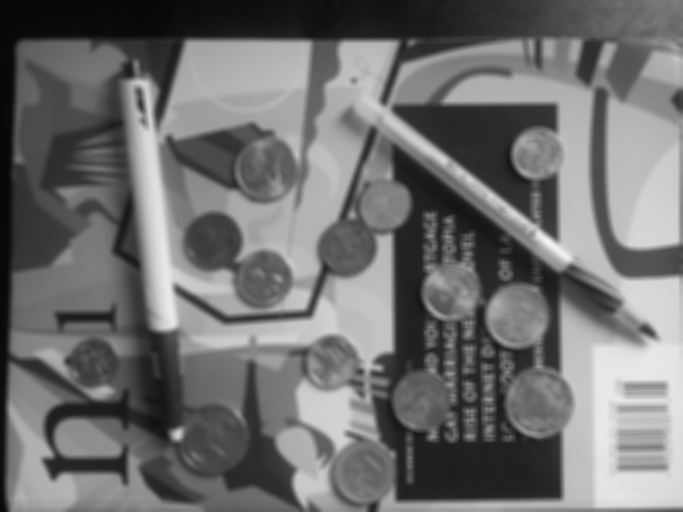
\includegraphics[width = .5\textwidth]{ps1-7-image-noisy-smoothed.png}&
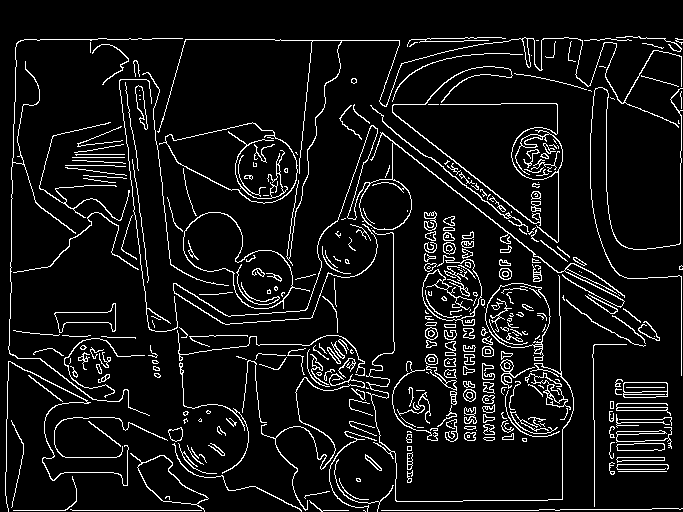
\includegraphics[width= .5\textwidth]{ps1-7-edges-image-noisy.png}\\
	a&b\\
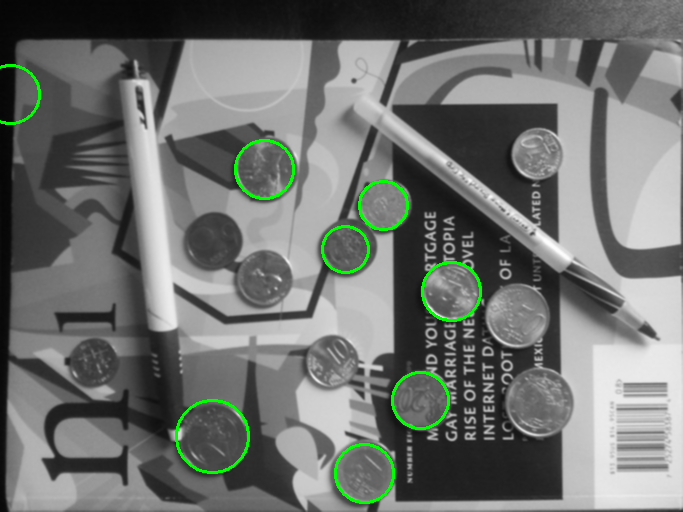
\includegraphics[width= .5\textwidth]{ps1-7-circles.png}\\	
\end{tabular}
\end{center}
 \caption{
\textit{a}. ps1-7-a-smoothed : Smoothed Image.  \textit{b}. ps1-7-a-edges : Edges Image Smoothed. 
\textit{c}. ps1-7-a-circles :  Hough Circles drawn on the smoothed image.}
\label{ps1-7}
\end{figure}

\section{Sensitivity to distortion}

\subsection{Application of the line and circles finder}

 \begin{figure}[H]
\begin{center}
\begin{tabular}{cc}
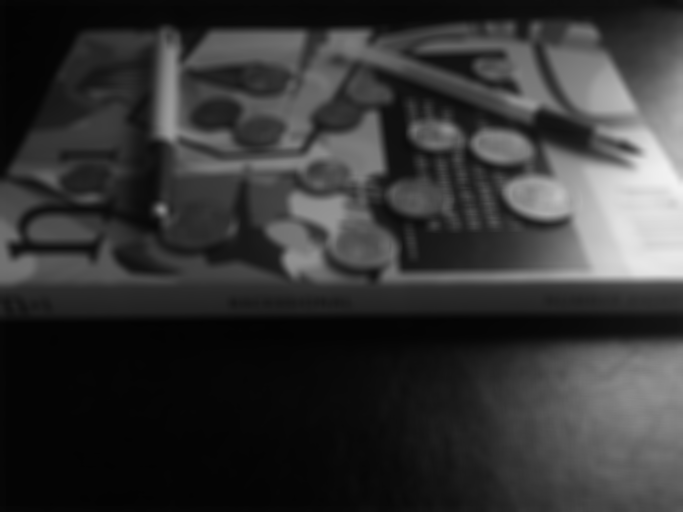
\includegraphics[width = .5\textwidth]{ps1-8-image-noisy-smoothed.png}&
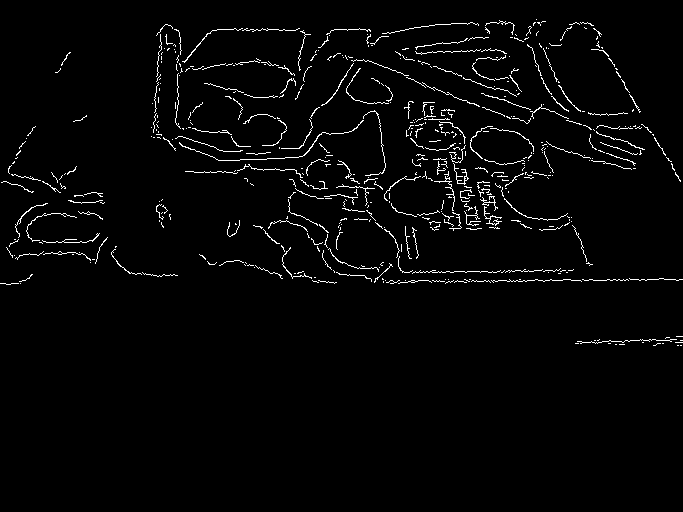
\includegraphics[width= .5\textwidth]{ps1-8-edges-image-noisy.png}\\
	a&b\\
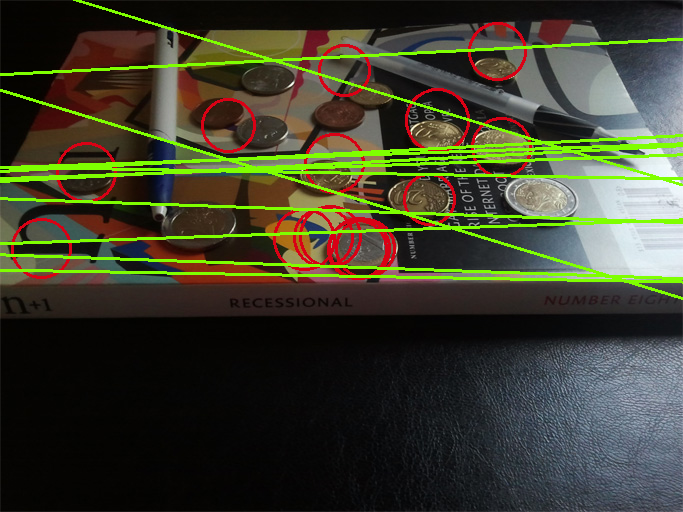
\includegraphics[width= .5\textwidth]{ps1-8-circles.png}\\	
\end{tabular}
\end{center}
 \caption{
\textit{a}. ps1-7-a-smoothed : Smoothed Image.  \textit{b}. ps1-7-a-edges : Edges Image Smoothed. 
\textit{c}. ps1-7-a-circles :  Hough Circles and Hough Lines drawn on the smoothed image.}
\label{ps1-7}
\end{figure}

Our two Hough transforms applied to a distorted image do not perform well (Figure 13.a). Even with a parallel lines filtering, which should help detect the pens even in this setup, we do not manage to extract any of their boundaries
but still get unwanted edges.

However, the circles detection seems to perform slightly better, despite plenty of false alarms it seems that we detect several coins, as well as the false circle visible in the "n" letter.

\subsection{How to fix the problem ?}

In future enhancements of our program we might try to adapt the circle transform to detect ellipses. We would however probably face at least the same amount of false alarms as in the previous section, and would also need to implement further improvements.
Regarding the lines, we would need to adapt the smoothing and edge detection to also take into account the stronger impact of the shadows on this distorted version of the image. We could also add constraints on the filtered lines to look for lines at specific angles and with a specific number of close parallel edges.

\end{document}